% Copyright (C)  2015  Alexander Jankowski, Philipp Hacker.
% Permission is granted to copy, distribute and/or modify this document
% under the terms of the GNU Free Documentation License, Version 1.3
% or any later version published by the Free Software Foundation;
% with no Invariant Sections, no Front-Cover Texts, and no Back-Cover Texts.
% The lincense itself can be found at <https://www.gnu.org/licenses/fdl-1.3>.

\documentclass[numbers=noenddot,a4paper,notitlepage,twoside,BCOR15mm]{scrartcl}
%\documentclass[numbers=noenddot,12pt,a4paper]{scrartcl}

\usepackage{ifoddpage}
\usepackage[infoshow]{tabularx}
\usepackage{fancyhdr}
\usepackage[greek,ngerman]{babel}
\usepackage[T1]{fontenc}
\usepackage[utf8]{inputenc}
\usepackage{libertine}
\usepackage{ziffer}
\usepackage{graphicx}
\usepackage{units}
\usepackage[infoshow]{tabularx}
\usepackage[all]{xy}
\usepackage{amsmath}
\usepackage{amssymb}
\usepackage{wrapfig}
\usepackage{upgreek}
\usepackage{esint}
\usepackage{float}
\usepackage[font=small,labelfont=bf]{caption}
\usepackage{subcaption}
\usepackage{lscape}
\usepackage[backref=page]{hyperref}
\usepackage{cleveref}
\usepackage{csquotes}

\renewcommand{\headrulewidth}{0.1pt}
\renewcommand{\footrulewidth}{0.1pt}
\newcommand{\name}{\text{Philipp Hacker}} %TODO Name des Protokollanten eintragen

\renewcaptionname{ngerman}{\figurename}{Abb. }
\renewcaptionname{ngerman}{\tablename}{Tab.}

\setlength{\parindent}{0pt}

\newcommand{\nummat}[1]{\left[\text{#1}\right]}
\newcommand{\num}[1]{$\left[\text{#1}\right]$}
\newcommand{\degree}{^\circ}
\newcommand{\diff}{\textnormal{d}}
\newcommand{\tenpo}[1]{ 10^{#1}}
\newcommand{\greek}[1]{\greektext#1\latintext}
\newcommand{\ix}[1]{_\text{#1}}
\newcommand{\imag}{\mathbf{i}}
\newcommand{\tilt}[1]{\textit{#1}}
\newcommand{\grad}[1]{\textit{grad}\left(#1\right)}
\newcommand{\divergenz}[1]{\textit{div}\left(#1\right)}
\newcommand{\euler}{\mathnormal{e}}
\newcommand{\fett}[1]{\textbf{#1}}
\newcommand{\einnup}{\hspace{0.2cm}}
\newcommand{\einnum}{\hspace{-0.2cm}}
\newcommand{\zentriert}[1]{\begin{center}#1\end{center}}

\title{Protokoll:OH-Rotationsspektroskopie} %TODO Name des Versuchs eintragen
\author{Alexander Jankowski, Philipp Hacker}
\date{\today}
\pagestyle{fancy}
\fancyhead[C]{\thepage}
\fancyhead[R]{\name}
\fancyfoot[C]{\thepage}
\fancyhead[L]{Abschnitt \thesection}

\begin{document}
	\maketitle
	\begin{center}
		Betreuer: \\ %TODO Name des Betreuers eintragen
		Versuchsdatum: 11.11.2015\\ %TODO Datum des Versuchs eintragen
		\begin{table}[h]
			\centering
			Note: %TODO Gute Note erhalten :)
			\begin{tabularx}{1.5cm}{|X|}
				\hline \\ \\
				\hline
			\end{tabularx}
		\end{table}
	\end{center}
	\vspace*{\fill}
	\tableofcontents
	\vfill
	\newpage
	\section{Motivation}
	
	\newpage
	\section{Physikalische Grundlagen}
	
	\newpage
	\section{Durchführung}
	
	\newpage
	\section{Auswertung}

		\subsection{Simulierte Spektren}

		\subsection{Reale Spektren}

				\begin{figure}
					\centering
					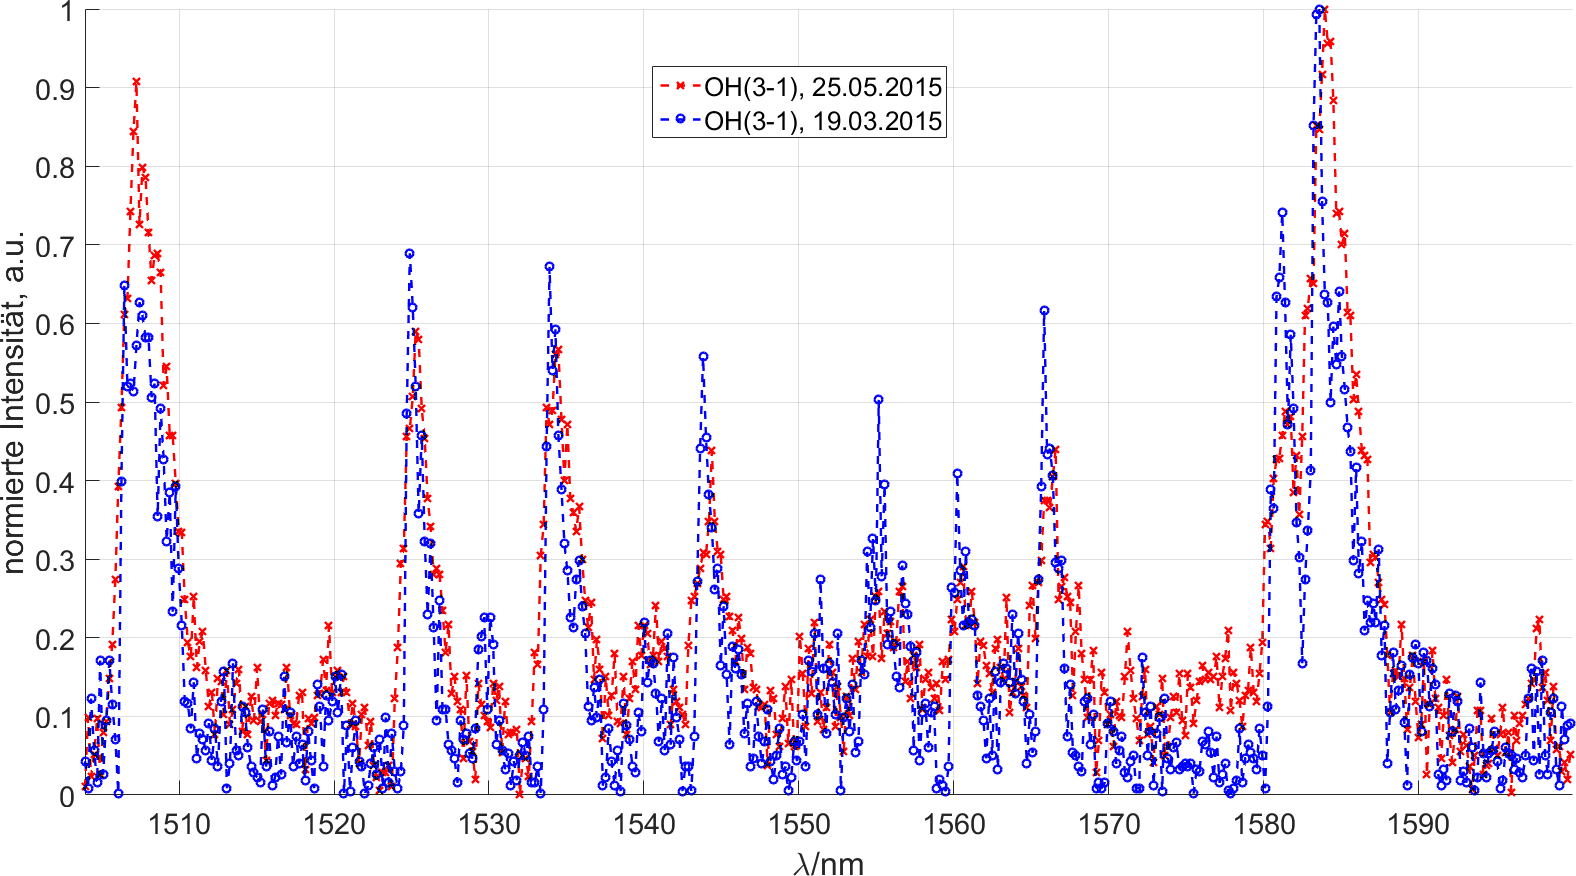
\includegraphics[width=0.9\textwidth]{spektr_unsmooth.png}
					\caption{Betrag der Differenz aus gemessenem Spektrum und Dunkelstrom-Intensität $|I-I\ix{0}|$. Gezeigt sind Verläufe vom 25.05. und 19.03.2015.}
					\label{img:spektr1}
				\end{figure}

				\begin{align}
					&y^{(s)}\ix{i}=\frac{y\ix{i-3}+y\ix{i-2}+y\ix{i-1}+y\ix{i}+y\ix{i+1}+y\ix{i+2}+y\ix{i+3}}{7} \label{eq:glatt} \\
					\text{wobei:} \quad &y^{(s)}\ix{1}=\frac{y\ix{1}+y\ix{2}+y\ix{3}+y\ix{4}}{4} \quad \text{usw.}\\
					\text{und} \quad &y^{(s)}\ix{N}=\frac{y\ix{N-3}+y\ix{N-2}+y\ix{N-1}+y\ix{N}}{4}
				\end{align}

				\begin{align}
					y\ix{i}=\frac{||I\ix{i}-I\ix{0,i}||}{\text{sup}\left\lbrace ||I\ix{i}-I\ix{0,i}||\right\rbrace\ix{i=0}^{N}}
				\end{align}

				\begin{figure}
					\centering
					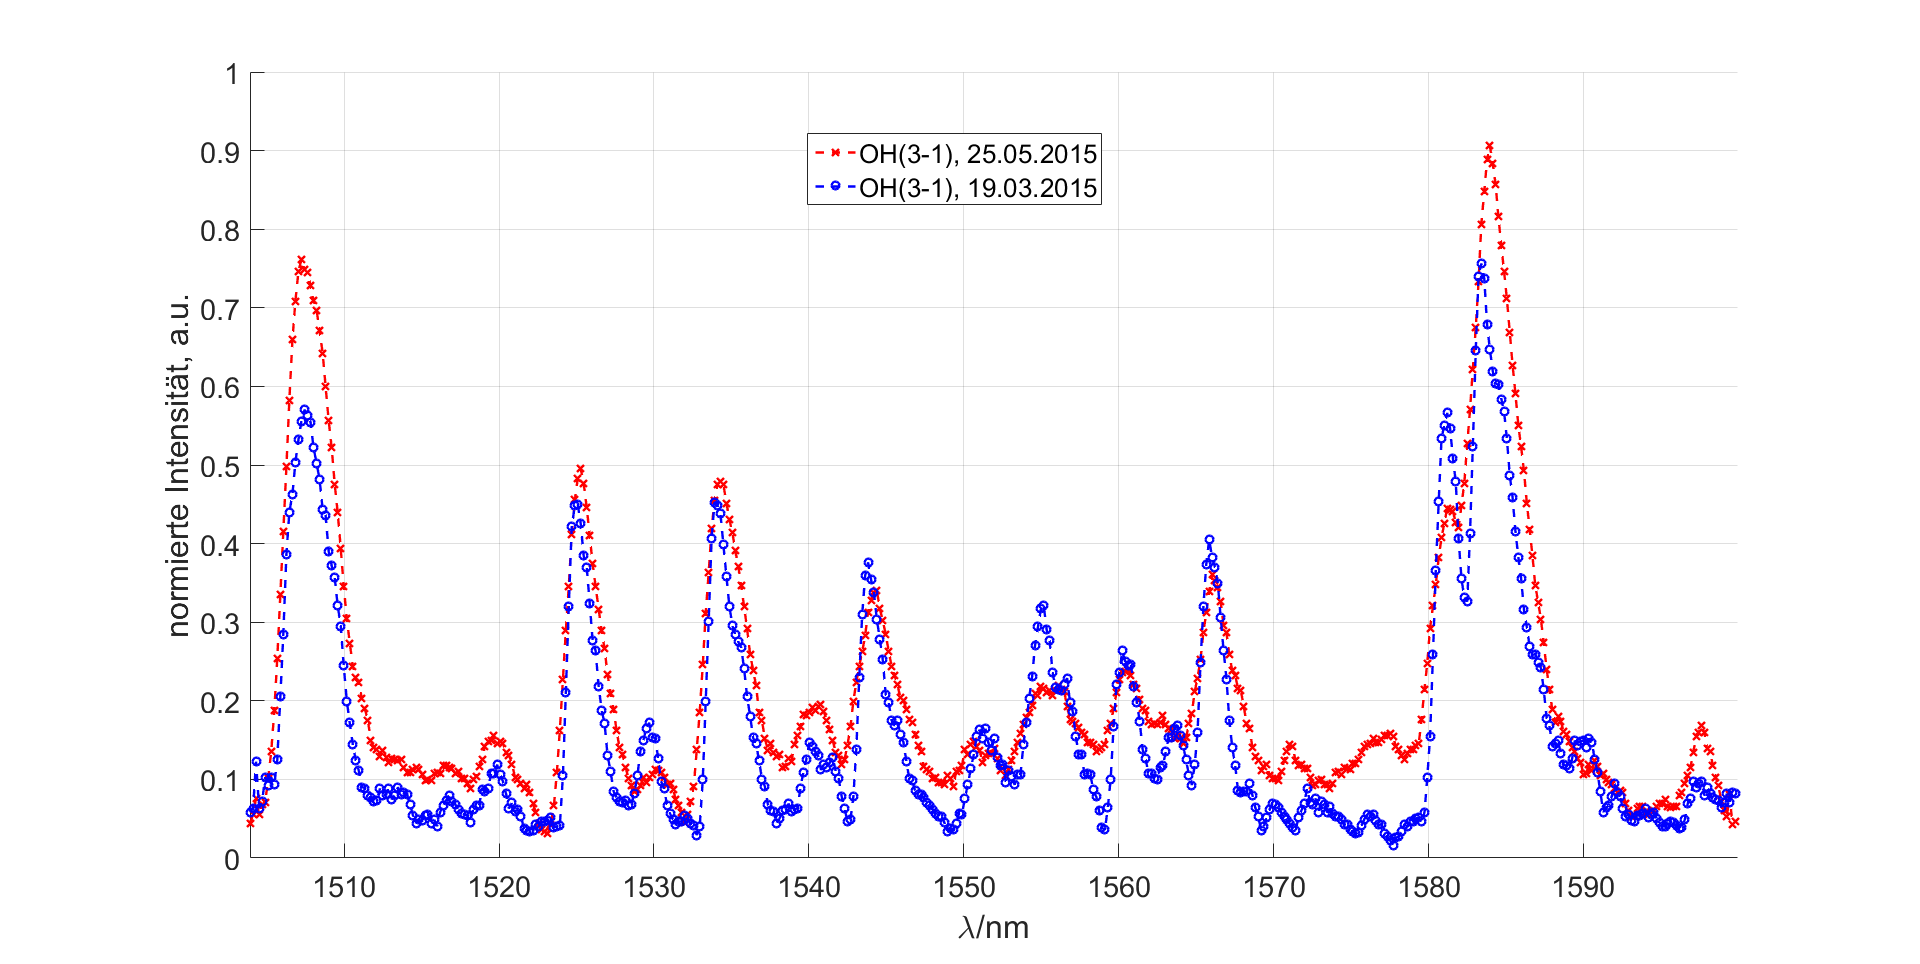
\includegraphics[width=0.9\textwidth]{spektr_smooth.png}
					\caption{Gleiche Daten wie in \autoref{img:spektr1} (Spektrum A, Spektrum B). Hier mit Hilfe einer polynomischen Glättung, maximal der Ordnung 7 verbessert. Der Zusammenhang kommt auf \autoref{eq:glatt}}
					\label{img:spektr2}
				\end{figure}

			\begin{table}
				\centering
				\begin{tabular}{c|c|c|c}
					Peaknummer & $\lambda/\unit[\tenpo{3}]{nm}$, aus \cite{EMAUGreifswaldOHRot} & $\lambda/\unit[\tenpo{3}]{nm}$, A & $\lambda/\unit[\tenpo{3}]{nm}$, B\\
					\hline $P\ix{1}(2)$ & 1,524 & 1,526 & 1,525 \\
					\hline $P\ix{1}(3)$ & 1,533 & 1,535 & 1,534 \\
					\hline $P\ix{1}(4)$ & 1,543 & 1,545 & 1,544
				\end{tabular}
				\caption{Wellenlängen der Peaks $P\ix{1}(2-4)$ im Vergleich zum Literaturwert aus \cite{EMAUGreifswaldOHRot}. Außerdem Gegenüberstellung der Werte aus den Intensitäten zum Spektrum A und B.}
				\label{tab:wellen}
			\end{table}

			\begin{table}
				\centering
				\begin{tabular}{c|c|c}
					Peaknummer & $|I-I\ix{0}|/\tenpo{2}$, zu A & $|I-I\ix{0}|/\tenpo{2}$, zu B\\
					\hline $P\ix{1}(2)$ & 2,993 & 1,995 \\
					\hline $P\ix{1}(3)$ & 2,873 & 1,945 \\
					\hline $P\ix{1}(4)$ & 2,223 & 1,615
				\end{tabular}
				\caption{Höhen der Peaks $P\ix{1}(2-4)$ an den Positionen aus \autoref{tab:wellen}. Gegenüberstellung von Spektrum A und B. Diese Werte sind für die Auswertung mit der linearen Regression aus \autoref{eq:linreg} wichtig.}
				\label{tab:intens}
			\end{table}

				\begin{figure}
					\centering
					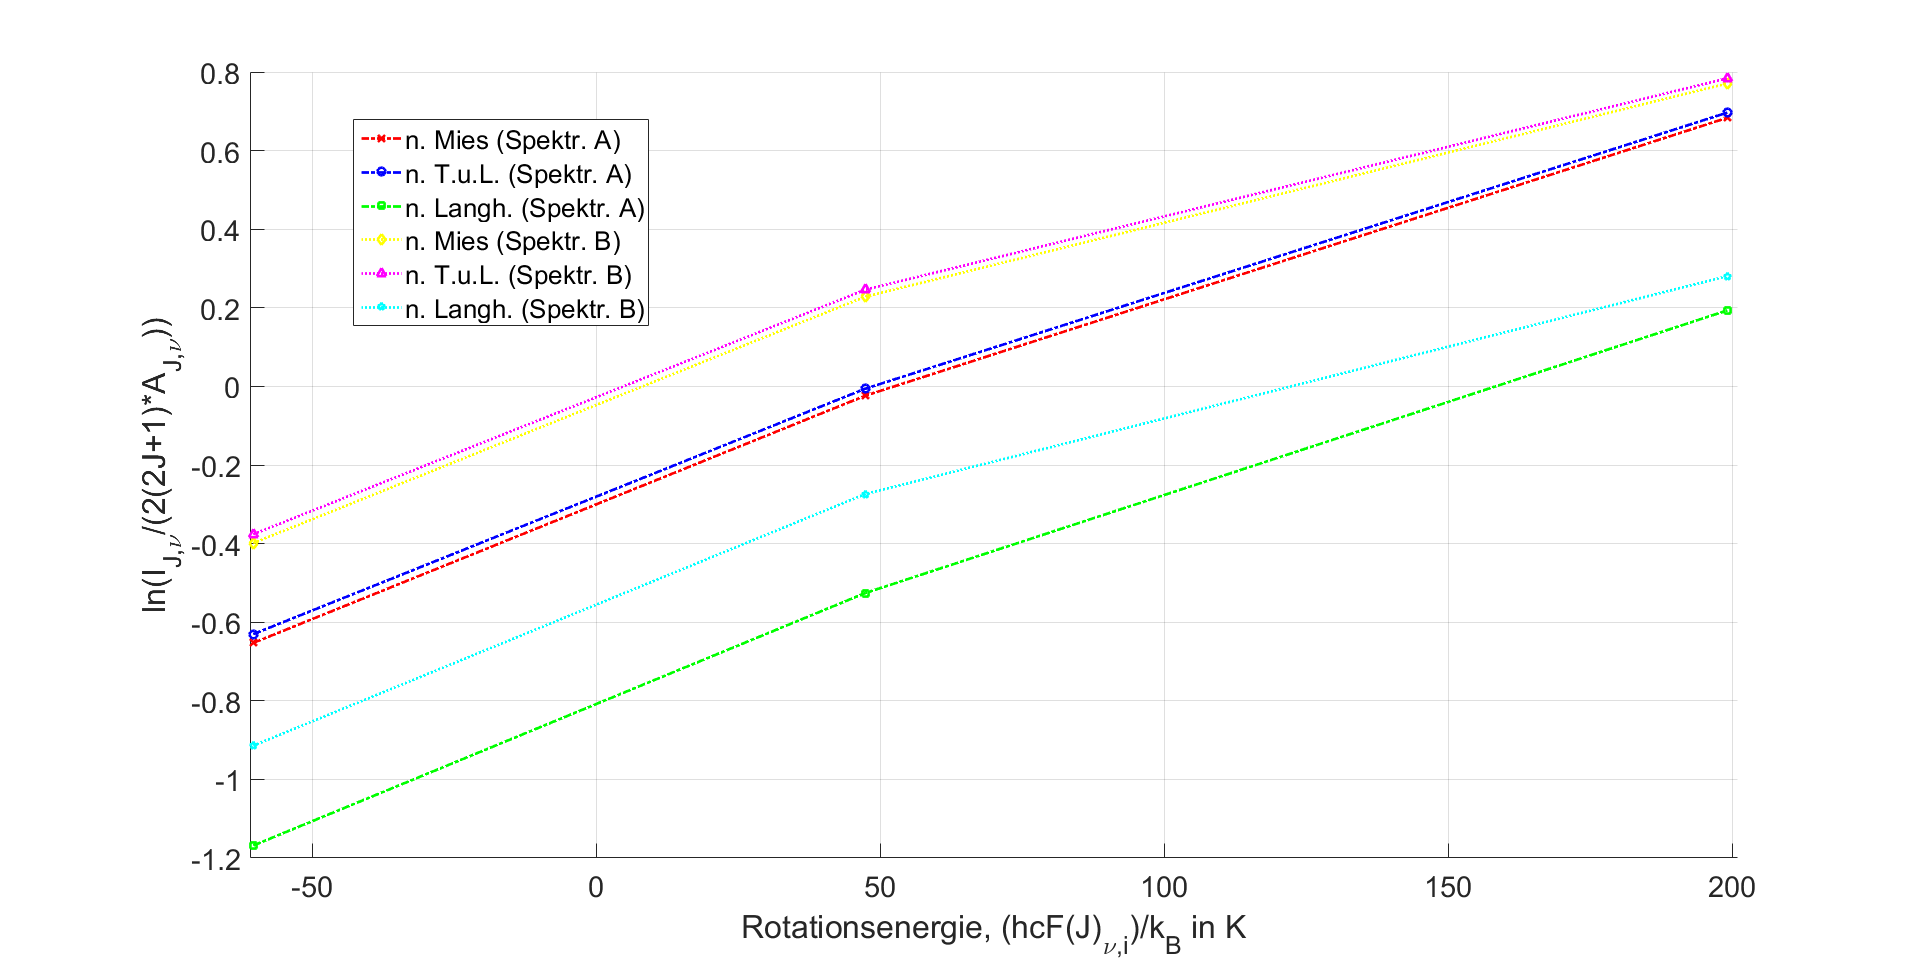
\includegraphics[width=0.9\textwidth]{linear_reg.png}
					\caption{Lineare Regression über die Rotationsenergie und Daten aus \autoref{tab:intens}.}
					\label{img:regress}
				\end{figure}

			\begin{table}
				\centering
				\begin{tabular}{c|c|c}
					Einsteinkoeffizienten, aus \cite{EMAUGreifswaldOHRot} & $T\ix{rot}/\unit{K}$, zu A & $T\ix{rot}/\unit{K}$, zu B\\
					\hline Mies (1947) & 347,98 & 241,75 \\
					\hline Turnbull u. Lowe (1989) & 342,44 & 239,06 \\
					\hline Langhoff (1986) & 1120,1 & 463,93
				\end{tabular}
				\caption{Rotationstemperaturen nach \autoref{eq:linreg}. Die Fehler nach Gauß sind in \autoref{eq:err} angegeben. Für die Intensität wurde das Dunkelstromkorrigierte Spektrum $|I-I\ix{0}|$ benutzt.}
				\label{tab:trot}
			\end{table}

		\subsection{Fehlerrechnung}

			\begin{figure}
				\centering
				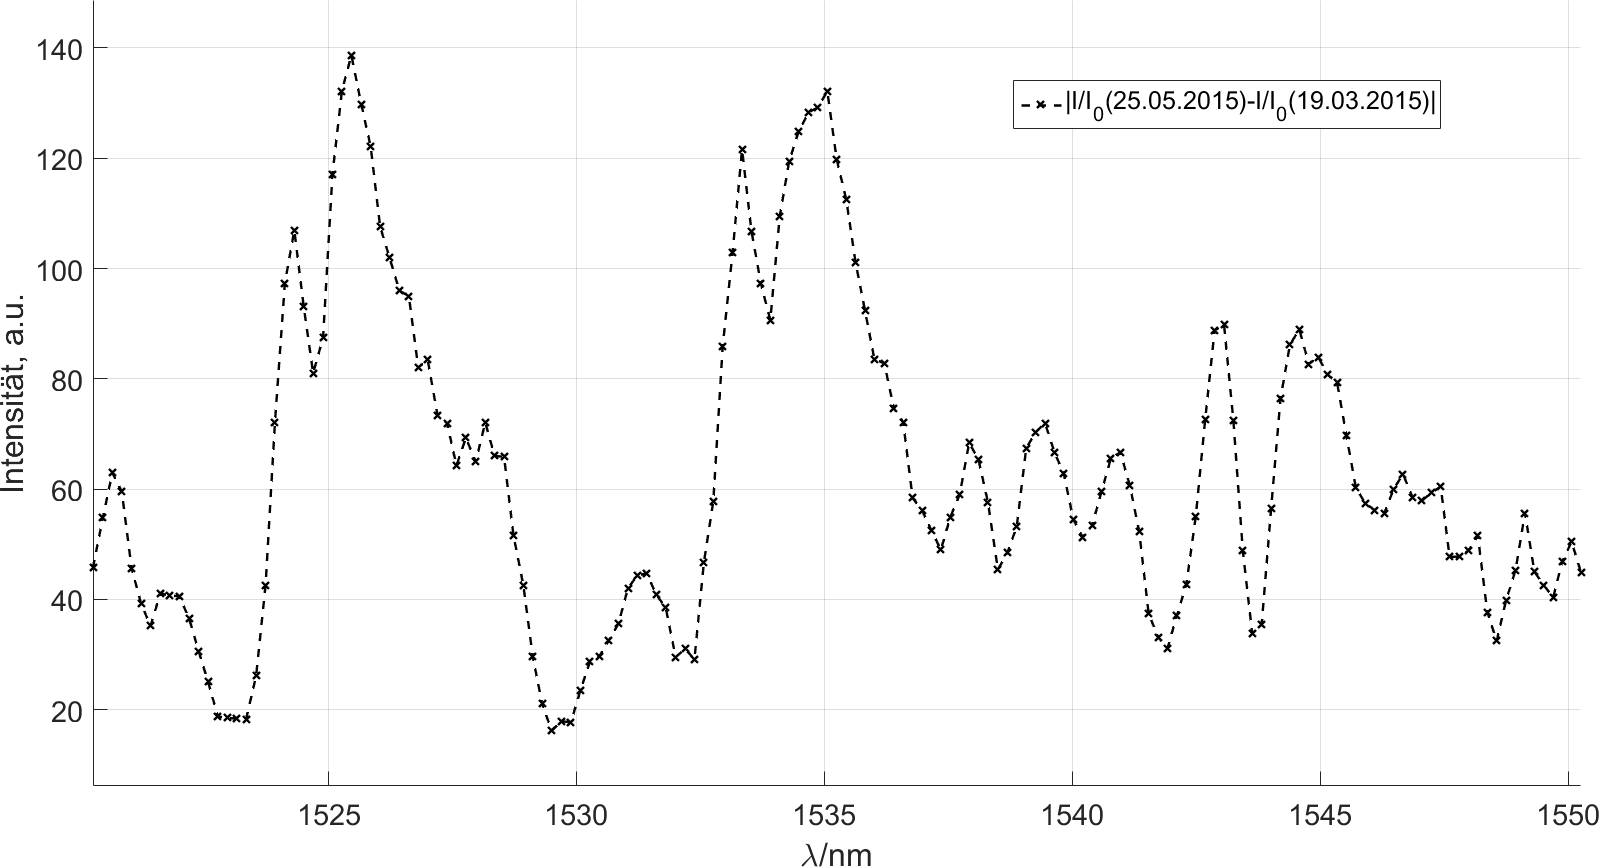
\includegraphics[width=0.9\textwidth]{differenz.png}
				\caption{Differenz aus Spektrum A und B. Ebenso wie \autoref{img:spektr2} über Polynome geglättet.}
				\label{img:diff}
			\end{figure}

			\begin{align}
				T\ix{rot}\left(I,\nu,i,J\right)\propto-&\frac{hcF\left(J,\nu,i\right)}{k\ix{B}}\ln\left(\frac{I\left(\nu,i,J\leftarrow\nu\prime,i\prime,J\prime\right)}{2\left(2J+1\right)A\left(\nu,i,J\rightarrow\nu\prime,i\prime,J\prime\right)}\right)^{-1} \\
				\Delta& T\ix{rot}\approx\sqrt{\left(\frac{\diff T\ix{rot}}{\diff I_{\nu,i,J}}\right)^2\cdot\left(\Delta I_{\nu,i,J}\right)^2} \label{eq:gauss}
			\end{align}

			\begin{align}
				\text{nach Mies:} \quad &T\ix{rot,A}=\left(347,98\pm 0,0424(11)\right)\unit{K} \label{eq:err}\\
				&T\ix{rot,B}=\left(241,75\pm 0,223(22)\right)\unit{K}
			\end{align}

			\begin{align}
				\text{nach Mies:} \quad &T^{(A)}\ix{rot,true}\in\left[347,67(03)\unit{K},348,29(02)\unit{K}\right] \\
				&T^{(B)}\ix{rot,true}\in\left[241,57(63)\unit{K},241,92(90)\unit{K}\right]
			\end{align}

	\newpage
	\section{Anhang}

		\bibliography{all.bib}
		\bibliographystyle{unsrt}

\end{document}